%%%%%%%%%%%%%%%%%%%%%%%%%%%%%%%%%%%%%%%%%%%%%%%%%%

\section{Domain Design of \hpl}
\label{sec:domainDesign}

This section introduces the domain design~\cite{gpbook} of \hpl. We begin with an architectural view (Section~\ref{sec:hpl-architecture}). Then, we describe \hpl's transformational approach to variability management (Section~\ref{sec:hpl-transformation}), which also relies on designated configuration knowledge (Section~\ref{sec:hpl-ck}), and a derivation process for SPL tools (Section~\ref{sec:hpl-derivation}).  Finally, bootstrapping of \hpl{} is described (Section~\ref{sec:hpl-bootstrapping}).

%%%%%%%%%%%%%%%%%%%%%%%%%%%%%%%%%%%%%%%%%%%%%%%%%%

\begin{figure*}[t!]
\begin{center}
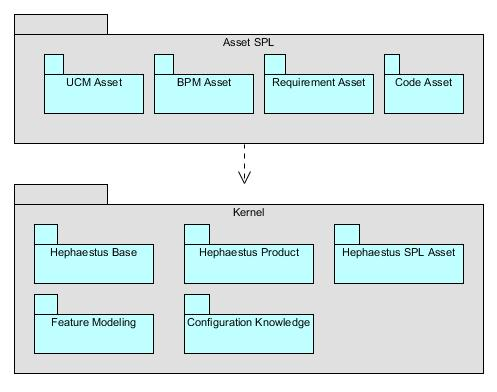
\includegraphics[width=.9\textwidth]{imagens/architecture-hpl-vf.jpg}
\end{center}
\caption{\hpl's architecture}
\label{fig:hpl-architecture}
\end{figure*}

%%%%%%%%%%%%%%%%%%%%%%%%%%%%%%%%%%%%%%%%%%%%%%%%%%

\subsection{\hpl's Architecture} 
\label{sec:hpl-architecture}

\hpl's architecture is depicted in Figure~\ref{fig:hpl-architecture}. Overall, \hpl{} is componentized in a way that most parts are separately compilable and unaffected by configuration or extension.

\emph{Kernel} represents the basic abstractions necessary for the generation of \hpl{} instances including the generation of \hpl{} itself in a bootstrapping process. Within the kernel, component \hpbase{} represents the commonality among all \hpl{} instances (as identified in Section~\ref{sec:commonality}); it serves as a base for deriving all \hpl{} instances. To this end, \hpbase{} has variability points (as identified in Section~\ref{sec:variability}) which are to be resolved by transformations defined in component \hpsplasset{} in a derivation process driven by component \hpproduct. These components of the kernel had to be specifically designed and implemented for \hpl. The kernel also hosts \emph{Feature Modeling} and \emph{Configuration Knowledge}: these components provide
basic abstractions for the representation of feature models, feature configurations, configuration knowledge as well as associated support functionality, e.g., for verifying validity of feature configurations relative to a given feature model. These components of the kernel could be reused from \hp{} and all \hpl{} instances share them, as is.

\textit{SPL Assets} represents the assets of \hpl. Each such \emph{meta-level} asset essentially corresponds to a type of artifact that can be targeted with an \hpl{} instance including the corresponding (non-meta-level) asset base for the type and designated support for variability management and product derivation in the domain of the asset. Each meta-level asset is essentially packaged in a component that exposes abstractions corresponding to the variation points of Section~\ref{sec:variability}: datatypes for the representation of assets and their transformation, functions for the interpretation of transformations, and other functionality related to \hpl's feature model, notably export functions.

%%%%%%%%%%%%%%%%%%%%%%%%%%%%%%%%%%%%%%%%%%%%%%%%%%

\subsection{\hpl's Transformational Approach} 
\label{sec:hpl-transformation}

We adopt a transformational approach~\cite{deltaSchaefer} to variability management. That is, the derivation of an \hpl{} instance involves source-code transformation. The approach provides transformations to address the heterogeneity of the variability patterns observed in Section~\ref{sec:hp-evolution} without compromising modularity and comprehensibility of \hpl, and thus configurability and extensibility, which may be issues for annotative approaches~\cite{kastner:2008}. The approach is also designed for uniformity. That is, the \hp{} approach to feature modeling, feature configuration, declaration and interpretation of configuration knowledge is adopted also at the meta-level. \hp{} often delegates some part of variability management to external tool support (e.g., for pre-processsing or aspect weaving), in which case, the transformation in the configuration knowledge essentially trigger those external transformations. In contrast, \hpl{} fully implements the meta-level transformations as metaprograms in Haskell on top of object programs in Haskell.

%%%%%%%%%%%%%%%%%%%%%%%%%%%%%%%%%%%%%%%%%%%%%%%%%%

\begin{figure}[t!]
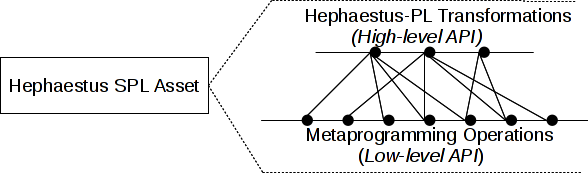
\includegraphics[scale=0.7]{imagens/apis-hpl-asset.png}
\caption{API levels for \hpsplasset}
\label{fig:hpl-apis}
\end{figure}

%%%%%%%%%%%%%%%%%%%%%%%%%%%%%%%%%%%%%%%%%%%%%%%%%%

Configuration of \hpl{} relies on transformations provided by a high-level API, which are implemented in terms of 
transformations of a low-level API, which, in turn, are implemented in terms of metaprogramming operations (with Haskell used both for object- and metaprograms).  The design of the high-level API captures the variability as identified during the domain analysis (Section~\ref{sec:variability}). The low-level API captures adaptation patterns as identified during the examination of the evolution scenario (Section~\ref{sec:hp-evolution}). Figure~\ref{fig:hpl-apis} illustrates the API layers, as they are part of \hpl's component \hpsplasset{} in the \emph{Kernel}. We refer to  Section~\ref{sec:metaprogrammingOperations} for the description of the actual implementation.

The transformations of the high-level API are described in the sequel. They are of specific interest, as they are directly used in the configuration of \hpl. 

\begin{description}

\item[SelectBase] The transformation selects \hpbase{}, which represents the commonality of all \hpl{} instances.
Typically, this is the first transformation to be executed in the process of deriving an instance. The implementation of \hpbase{} is given in Section~\ref{sec:hpbase}.

\item[SelectAsset] refines the product being derived with support for the selected asset variability as described by the feature configuration, i.e., this transformation extends the \texttt{SPLModel}, \texttt{InstanceModel} and \texttt{TransformationModel} data types and the \texttt{transform}, \texttt{xml2Transformation}, and \texttt{mkEmptyInstance} (empty instance definition to \texttt{build} function) functions to manipulate such asset. Furthermore, it incorporates the modules defining algebraic data types, the transformations, and the parser of the selected asset in the product being derived.  It also performs extensions into \texttt{main} function introducing the asset parser instruction and extending the instance of \texttt{SPLModel} data type with the asset selected to the \texttt{build} process.

\item[SelectExport] refines the product being derived with support for the selected output format by extending the \texttt{ExportModel} data type, the \texttt{lstExport} list definition and the \texttt{export} function. Furthermore, it incorporates the module implementing the selected output format function into the product being derived. We define different transformations as \texttt{SelectAsset} and \texttt{SelectExport} to represent the refinement on the base product because the set of metaprogramming operations associated with each of these \hpl{} transformations is different and independent.

\item[BindProductName] sets \hpl{}'s instance module name.

\item[RemoveProductMainFunction] is only used when the \hp{} feature is in a configuration of \hpl's FM. This transformation removes the definition of the \texttt{main} function from the product being derived because the \hp{} feature uses the \texttt{buildHpl} function located in another module instead.

\item[SelectCKParser] refines the product being derived with the CK parser by introducing sentences into the \texttt{main} function to execute the parsing of \hpl's instance CK and changing the \texttt{product} declaration from \texttt{undefined} to \texttt{build fm fc cm spl}, which refers to the CK defined by the \texttt{SelectCKParser} transformation. Furthermore, it incorporates the module defining the CK XML parser into the emerging product. This transformation is only applied to the \texttt{NOT \hp{}} feature expression. When \texttt{\hp{}} feature is selected, such transformation is not applied because the instance corresponding to this feature is the \hp{} \emph{Product} and the transformations for managing variability within it are precisely the transformations described in this bullet list, which are referred to from the \hp{} \emph{Product} and thus do not need to be parsed.

\end{description}

When we build an \hpl{} instance, the derivation process first reads the \texttt{HephaestusBase} module and then performs \hp{} asset transformations (mainly \texttt{SelectAsset} and \texttt{SelectExport}), refining several definitions of the module. 

We defined six \hpl{} transformations, which are represented by the following type constructors:

%%%%%%%%%%%%%%%%%%%%%%%%%%%%%%%%%%%%%%%%%%%%%%%%%%

\begin{table}[h]
\begin{center}
\begin{tabular}{||l||l||}
  \hline
  \textbf{Feature Expressions} & \textbf{Transformations}   \\  \hline
  True & SelectBase \\  \hline
%  Hephaestus & BindProductName "Hephaestus" \\
%             &  SelectAsset "Hephaestus"   \\
%             &  RemoveProductMainFunction \\ \hline
%  NOT Hephaestus & SelectCKParser \\ \hline
  UseCase & SelectAsset "Use Case" \\ \hline
  UseCase AND UcmToXML & SelectExport "UcmToXML"  \\ \hline
  UseCase AND UcmToLatex & SelectExport "UcmToLatex" \\ \hline
  BusinessProcess & SelectAsset "Business Process" \\ \hline
  BusinessProcess AND BpmToXML & SelectExport "BpmToXML" \\ \hline
  Requirement & SelectAsset "Requirement" \\ \hline
  Requirement AND ReqToLatex & SelectExport "ReqToLatex" \\ \hline
  Code & SelectAsset "Code" \\ \hline
  Code AND BuildFile & SelectExport "BuildFile" \\ \hline
\end{tabular}
\caption{Excerpt of \hpl's Configuration Knowledge}
\label{tab:hpl-ck}
\end{center}
\end{table}

%%%%%%%%%%%%%%%%%%%%%%%%%%%%%%%%%%%%%%%%%%%%%%%%%%

\subsection{\hpl's Configuration Knowledge} 
\label{sec:hpl-ck}

%%%%%%%%%%%%%%%%%%%%%%%%%%%%%%%%%%%%%%%%%%%%%%%%%%

Figure~\ref{fig:derivationHPL} abstractly depicts the steps taken in \hpl's product derivation process considering the feature configuration shown in  Figure~\ref{fig:fc-ucm-bpm}. \hpl{}'s CK (Table~\ref{tab:ck-hpl}) guides this transformational process in five steps towards the generation of a \hpl{} instance from the base product. \hpl{}'s CK is evaluated from first to last row, triggering execution of only those transformations whose corresponding feature expression evaluates to true according to the given configuration.

%%%%%%%%%%%%%%%%%%%%%%%%%%%%%%%%%%%%%%%%%%%%%%%%%%

\begin{figure*}[t!]
\begin{center}
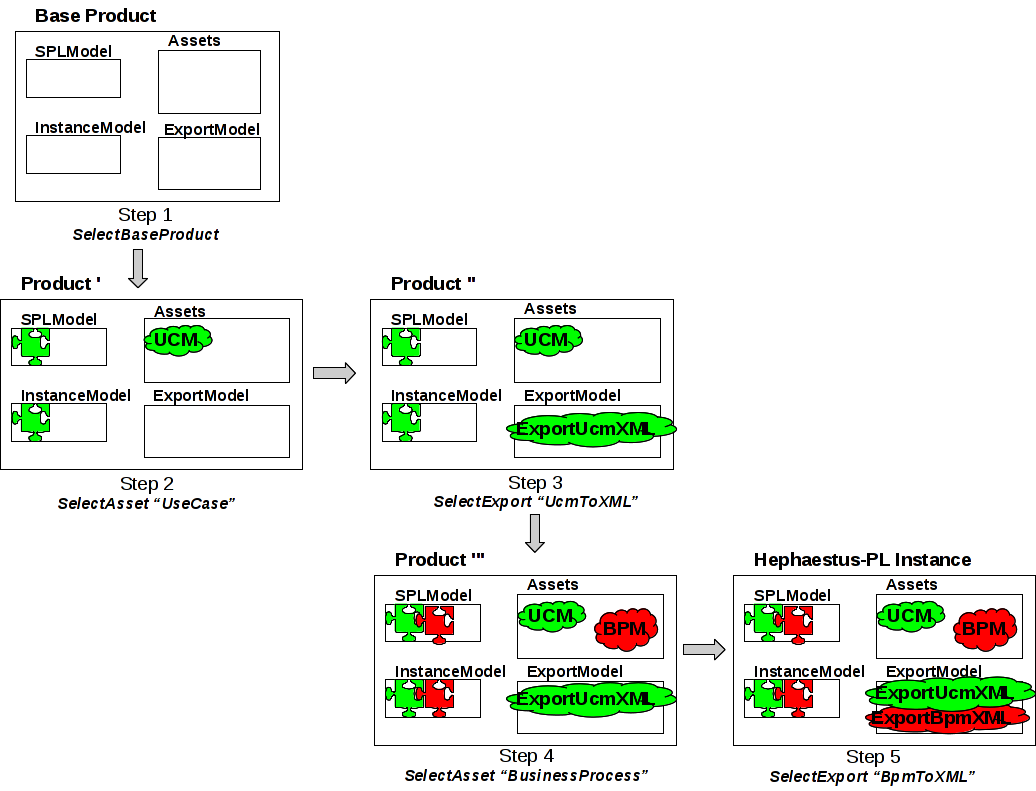
\includegraphics[width=\textwidth]{imagens/derivation.png}
\end{center}
\caption{Derivation of an \hpl{} instance supporting the UCM, BPM, UcmToXML and BpmToXML features.}
\label{fig:derivationHPL}
\end{figure*}

%%%%%%%%%%%%%%%%%%%%%%%%%%%%%%%%%%%%%%%%%%%%%%%%%%

\subsection{\hpl's Derivation Process} 
\label{sec:hpl-derivation}

To illustrate a key scenario of \hpl's product derivation process, suppose a specific feature configuration (FC) contains four features: use case model (\emph{UseCase}), business process model (\emph{BusinessProcess}), use case in xml format (\emph{UcmToXML}), and business process in xml format (\emph{BpmToXML}), as shown in the Figure~\ref{fig:fc-ucm-bpm}.

%%%%%%%%%%%%%%%%%%%%%%%%%%%%%%%%%%%%%%%%%%%%%%%%%%

\begin{figure*}[t!]
\begin{center}
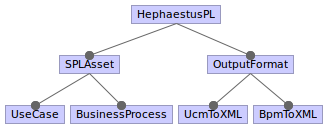
\includegraphics[scale=0.8]{imagens/fc-ucm-bpm.png}
\end{center}
\caption{\hpl's feature configuration to generate a \hpl's instance}
\label{fig:fc-ucm-bpm}
\end{figure*}

%%%%%%%%%%%%%%%%%%%%%%%%%%%%%%%%%%%%%%%%%%%%%%%%%%

\hpl's product derivation process is based on \hpl's Configuration Knowledge (CK), an excerpt of which is shown in Table~\ref{tab:ck-hpl}.  This CK relates feature expressions to transformations that solve \hpl{}'s variability.  As shown in the \textit{transformations} column of Table~\ref{tab:ck-hpl}, we defined \hpl's transformations which are detailed in Subsection~\ref{hp-spl-asset}, and when applied they progressively bind variability in the base product (cf. Figure~\ref{fig:derivationHPL}) as \hpl's instance is generated.

Accordingly, \hpl's product derivation process begins with the execution of the \texttt{SelectBase} transformation associated with the feature expression \texttt{True} in the first line of \hpl's CK (Table ~\ref{tab:ck-hpl}). Indeed, this transformation is always executed at the beginning of the generation of a new \hpl{} instance and represents the selection of the base product that contains the commonality of any \hpl{} instance.

Next, in the second line of \hpl's CK, the \texttt{UseCase} feature expression evaluates to true according to the FC shown in Figure~\ref{fig:fc-ucm-bpm} and thus the \texttt{SelectAsset "Use Case"} transformation is executed: it performs a set of transformations in the base product, binding variation points of the base product by adding components of the \textit{UCM Asset}(Step 2 in Figure~\ref{fig:derivationHPL}).  More specifically, the transformation introduces the UCM asset data type as field into the \texttt{SPLModel} and \texttt{InstanceModel} data types and imports the modules that define the UCM data types and corresponding transformations.  Following in the Step 3, feature expression \texttt{UseCase AND UcmToXML} evaluates to true in the third line of \hpl's CK and then the \texttt{SelectExport "UcmToXML"} transformation is executed. This transformation extends the product under derivation, adding components of the \textit{UCM Asset} to support the exportation of use cases in the XML format, i.e., introduces the \texttt{ExportUcmXML} constructor corresponding to \textit{UcmToXML} feature into \texttt{ExportModel} data type and adds the module that implements use case's xml output format into Product'.

Steps 4 and 5 then execute similar transformations in the product under derivation to those performed by Steps 2 and 3 described previously.  Therefore, the \texttt{BusinessProcess} and \texttt{BusinessProcess AND BpmToXML} feature expressions evaluate to true according to the configuration. As a result, the corresponding transformations in the CK bind some more of the remaining variation points of the product under derivation by adding components of the \textit{BPM Asset} into this product to support the variability management and export capability of business process model in the generated \hpl{} instance.

We note that both \textit{UCM Asset} and \textit{BPM Asset} are architectural elements belonging to \textit{SPL Assets}, as represented in Figure~\ref{fig:architecture-hpl}.

%%%%%%%%%%%%%%%%%%%%%%%%%%%%%%%%%%%%%%%%%%%%%%%%%%

%\subsection{\hpl's Architectural Elements} \label{architectural-elements-hpl}

In what follows we detail the main building blocks of \hpl{}'s architecture with emphasis on the kernel and its related elements (Core Assets and SPL Assets).  The kernel consists of three elements: \hp{} Product (Section~\ref{hp-product}), \hp{} SPL Asset (Section~\ref{hp-spl-asset}), and \hp{} \emph{Base} (Section~\ref{hp-base}). Together these elements comprise the minimal structure responsible for generating instances of \hpl{} products. Further, they have a certain degree of coupling and are mostly stable with respect to evolution of \hpl{}. Sections~\ref{spl-assets} and~\ref{core-assets} describe SPL Assets and Core Assets, respectively.

%%%%%%%%%%%%%%%%%%%%%%%%%%%%%%%%%%%%%%%%%%%%%%%%%%

\subsubsection{\hp{} Product} 
\label{hp-product}


Managing variability of \hp{} SPL Asset means that \hp{} \emph{Product} is used to derive products according to \hpl{}'s variability space. In particular, the module provides the \texttt{build} function, which controls \hpl{}'s product derivation process--by progressive refinement of the base product.

%%%%%%%%%%%%%%%%%%%%%%%%%%%%%%%%%%%%%%%%%%%%%%%%%%

\begin{figure}
\begin{lstlisting}
data HephaestusModel = HephaestusModel [HsModule]

data HephaestusTransformation = SelectBase
                              | SelectAsset String
                              | SelectExport String
                              | BindProductName String
                              | RemoveProductMainFunction
                              | SelectCKParser

transformHpl :: HephaestusTransformation
             -> SPLModel
             -> InstanceModel
             -> InstanceModel
\end{lstlisting}
\caption{Code snippet of the Hephaestus SPL Asset}
\label{fig:code-hp-spl-asset}
\end{figure}

%%%%%%%%%%%%%%%%%%%%%%%%%%%%%%%%%%%%%%%%%%%%%%%%%%

\subsubsection{\hp{} SPL Asset} 
\label{hp-spl-asset}

This element declares algebraic data types representing \hp{} SPL asset, which just corresponds to a list of Haskell modules and the set of transformations for managing \hpl{} variability (code snippet in Figure~\ref{fig:code-hp-spl-asset}). In essence, these transformations are responsible for the refinement of the base product during derivation of the \hpl{} instance. In addition, this module also declares the \texttt{transformHpl} function which is responsible for actually performing the corresponding \hpl{} transformations and it has the same signature of \texttt{transform} function declared in the \hp{} product described in Section~\ref{hp-product}.


%%%%%%%%%%%%%%%%%%%%%%%%%%%%%%%%%%%%%%%%%%%%%%%%%%

%\subsubsection{SPL Assets} 
\label{spl-assets}

Define the artifacts for each SPL asset, i.e., the algebraic data types representing a SPL asset, the set of transformations for solving asset's variability and the parser function to convert the external format into algebraic data types defined to \hpl.

In addition, this module also needs to define a data type and a function that comprising all asset's transformations to be used in \texttt{transform} function in the refinement of the base product when the asset is selected, for example, \texttt{UseCaseTransformation} data type and \texttt{transformUcm} function to the \texttt{Use Case} asset. The \texttt{transformUcm} function must have the same signature of \texttt{transform} function declared in the base product described in Section~\ref{base-product}.

%%%%%%%%%%%%%%%%%%%%%%%%%%%%%%%%%%%%%%%%%%%%%%%%%%

%\subsubsection{Core Assets} \label{core-assets}

The instances of the \hpl{}'s FM and CK are key inputs in the \texttt{build} process of \textit{\hp{} Product} to derive new \hpl{} instances.

The \hpl{}'s FM declares the variability space of \hpl{}, as shown in Figure~\ref{fig:hp-fm-03}. The whole \hpl{'s} CK is represented by Table~\ref{tab:ck-hpl} adding the lines related to \texttt{\hp{}} feature as shown in the Table~\ref{tab:ck-hpl-2}.

%%%%%%%%%%%%%%%%%%%%%%%%%%%%%%%%%%%%%%%%%%%%%%%%%%

\begin{table}[h]
\begin{center}
\begin{tabular}{||l||l||}
  \hline
  \textbf{Feature Expressions} & \textbf{Transformations}   \\  \hline
  Hephaestus & BindProductName "Hephaestus" \\
             &  SelectAsset "Hephaestus"   \\
             &  RemoveProductMainFunction \\ \hline
  NOT Hephaestus & SelectCKParser \\ \hline
\end{tabular}
\caption{Lines of \hpl's CK related to \texttt{\hp{}} feature}
\label{tab:ck-hpl-2}
\end{center}
\end{table}

%%%%%%%%%%%%%%%%%%%%%%%%%%%%%%%%%%%%%%%%%%%%%%%%%%

\subsection{Bootstrapping of \hpl} 
\label{sec:hpl-bootstrapping}

Whenever we want to bootstrap \hpl, we derive an instance of \hpl{} using a feature configuration that has only the \texttt{\hp{}} feature. This will trigger the product derivation of an instance that manages variability of the \hp{} asset. Differently, if we use a feature configuration that has both features \texttt{UseCase} and \texttt{BusinessProcess}, the product derivation will generate an \hpl{} instance that manages variability related to these assets.

\hpproduct{} is a minimal \hpl{} instance that only supports variability management of \hp{} \emph{SPL Asset} and corresponds to a Haskell module that could be generated by bootstrapping, i.e., \hp{} \emph{Product} could be used to generate itself, in which case the \hp{} feature is selected in a configuration of \hpl's FM. 

%%%%%%%%%%%%%%%%%%%%%%%%%%%%%%%%%%%%%%%%%%%%%%%%%%
